\documentclass[12pt,a4paper]{article}
\usepackage[utf8]{inputenc}
\usepackage[T1]{fontenc}
\usepackage{mathptmx}
\usepackage[brazil]{babel}
\usepackage{amsmath,amssymb}
\usepackage{booktabs}
\usepackage{longtable}
\usepackage{graphicx}
\usepackage[style=abnt,backend=biber,language=brazil,
            maxcitenames=2,maxbibnames=99,
            uniquename=false,giveninits=false]{biblatex}
\addbibresource{refs.bib}
\usepackage[hidelinks,pdfusetitle=false]{hyperref}
\hypersetup{
  pdftitle  = {Sa\'ida da Ford e Emprego Setorial no Brasil},
  pdfauthor = {}
}
\usepackage{geometry}
\geometry{top=2.5cm,bottom=2.5cm,left=2.5cm,right=2.5cm}
\usepackage{setspace}
\singlespacing

\begin{document}

% ============================================================
% PÁGINA 2 (versão anônima): TÍTULO, RESUMO, PALAVRAS-CHAVE E JEL
% ============================================================
\begin{center}
{\large\textbf{\'Area~1: Economia Regional}}

\bigskip

{\large\textbf{Sa\'ida da Ford e Emprego Setorial no Brasil: Estimativa DDD com
Efeitos Fixos, Estudo de Evento e Testes de Robustez}}
\end{center}

\bigskip

\noindent\textbf{Resumo:} Este artigo estima o efeito causal do encerramento das opera\c{c}\~oes industriais da Ford no Brasil, anunciado em 2021 e concentrado nas plantas de Cama\c{c}ari (BA), Taubat\'e (SP) e Horizonte (CE), sobre o emprego formal no complexo automotivo. Utilizam-se microdados administrativos da Rela\c{c}\~ao Anual de Informa\c{c}\~oes Sociais (RAIS) no per\'iodo entre 2014 e 2023, agregados ao n\'ivel munic\'ipio $\times$ setor $\times$ ano para permitir uma an\'alise microlocal. A estrat\'egia emp\'irica fundamenta-se no m\'etodo de Diferen\c{c}as em Diferen\c{c}as Tripla (DDD), explorando varia\c{c}\~oes simult\^aneas no tempo (pr\'e/p\'os-2021), no espa\c{c}o (munic\'ipios tratados versus n\~ao tratados) e no setor (complexo automotivo versus demais setores da economia). O modelo incorpora efeitos fixos de alta dimens\~ao (munic\'ipio--ano, setor--ano e munic\'ipio--setor) e erros-padr\~ao agrupados no n\'ivel municipal para garantir a robustez da infer\^encia estat\'istica. A estimativa principal \'e negativa e estatisticamente significativa ($\hat{\beta} = -1{,}3992$; $p = 0{,}0034$), implicando uma redu\c{c}\~ao de aproximadamente $75{,}3\%$ no emprego setorial formal nas localidades diretamente expostas ap\'os 2021. O estudo de evento indica a aus\^encia de din\^amicas diferenciais no pr\'e-tratamento e uma contra\c{c}\~ao persistente no per\'iodo p\'os-choque. Em conjunto, as evid\^encias apontam que a sa\'ida da montadora constituiu um choque econ\^omico local de grande magnitude, com impactos adversos duradouros sobre o mercado de trabalho formal.

\medskip
\noindent\textbf{Palavras-chave:} Sa\'ida da Ford do Brasil; Setor automotivo; Choque econ\^omico local; Mercado de trabalho; Diferen\c{c}as em Diferen\c{c}as Tripla.

\medskip
\noindent\textbf{Classifica\c{c}\~ao JEL:} J23, J65, C23.

\bigskip

\noindent\textbf{Abstract:} This paper estimates the causal effect of Ford's industrial shutdown in Brazil, announced in 2021 and concentrated in the manufacturing plants of Cama\c{c}ari (BA), Taubat\'e (SP), and Horizonte (CE), on formal employment within the automotive complex. We utilize administrative microdata from the Brazilian \textit{Rela\c{c}\~ao Anual de Informa\c{c}\~oes Sociais} (RAIS) for the 2014--2023 period, aggregated at the municipality $\times$ sector $\times$ year level to provide a precise micro-territorial analysis. The identification strategy relies on a triple-differences (DDD) design, exploiting simultaneous variation over time (pre/post-2021), across space (treated versus non-treated municipalities), and across sectors (automotive complex versus other economic sectors). The empirical specification includes high-dimensional fixed effects (municipality--year, sector--year, and municipality--sector) and municipality-clustered standard errors to ensure the robustness of the statistical inference. The main estimate is negative and statistically significant ($\hat{\beta} = -1.3992$; $p = 0.0034$), implying an approximate $75.3\%$ reduction in formal sectoral employment in the directly exposed locations after 2021. An event-study specification shows no differential dynamics prior to the treatment and a persistent contraction following the shock. Overall, the evidence suggests that Ford's exit represented a major local economic shock with persistent adverse effects on formal employment in the automotive complex in directly exposed areas.

\medskip
\noindent\textbf{Keywords:} Ford's Exit from Brazil; Automotive Sector; Local Economic Shock; Labor Market; Triple Differences-in-Differences.

\medskip
\noindent\textbf{JEL Code:} J23, J65, C23.

\clearpage

% ============================================================
\section{Introdu\c{c}\~ao}
\label{sec:intro}

O encerramento das opera\c{c}\~oes industriais da Ford no Brasil, anunciado em 2021 e envolvendo plantas em Cama\c{c}ari (BA), Taubat\'e (SP) e Horizonte (CE), constitui um choque econ\^omico local de grande magnitude, uma vez que altera abruptamente o n\'ivel de atividade e o mercado de trabalho de localidades com elevada depend\^encia de uma planta \^ancora. A literatura sobre o desenvolvimento regional enfatiza que a concentra\c{c}\~ao de atividades industriais em polos espec\'ificos tende a intensificar efeitos de polariza\c{c}\~ao e a vulnerabilidade territorial a choques idiossincr\'aticos \parencite{yeung2017}. No caso brasileiro, a implanta\c{c}\~ao e consolida\c{c}\~ao de complexos automotivos esteve associada \`a competi\c{c}\~ao locacional e a arranjos institucionais que nem sempre asseguram enraizamento produtivo no longo prazo.

A relev\^ancia deste estudo vai al\'em dos empregos diretos na montadora, pois o setor automotivo movimenta uma cadeia complexa de fornecedores e servi\c{c}os. Essa rede envolve encadeamentos como autopeças, metalurgia, pl\'asticos e manuten\c{c}\~ao, o que aumenta o potencial de efeitos negativos sobre a renda e o trabalho local. Pesquisas baseadas em simula\c{c}\~oes indicam que o fechamento das plantas gera perdas econ\^omicas significativas. Embora esses impactos sejam mais fortes nas cidades que abrigavam as f\'abricas, o preju\'izo acaba se espalhando por todos os elos da cadeia produtiva \parencite{domingues2020,fernandes2021}.

Em n\'ivel microlocal, a vulnerabilidade tende a ser maior quando o mercado de trabalho local \'e especializado e concentrado. Evid\^encia recente para Cama\c{c}ari (BA) indica elevada depend\^encia setorial e sugere que a especializa\c{c}\~ao ocupacional pode dificultar a realoca\c{c}\~ao r\'apida de trabalhadores na pr\'opria regi\~ao \parencite{henriques2024}. Em paralelo, resultados internacionais apontam que o efeito l\'iquido do fechamento depende do balan\c{c}o entre destrui\c{c}\~ao direta e capacidade de resposta do tecido produtivo local (expans\~ao de firmas incumbentes e entrada de novas firmas), o que torna indispens\'avel a mensura\c{c}\~ao emp\'irica do impacto observado \parencite{jofremonseny2018}.

A sa\'ida da Ford tamb\'em se sobrep\~oe a transforma\c{c}\~oes estruturais e tecnol\'ogicas do setor automotivo. S\'inteses recentes destacam oscila\c{c}\~oes de produ\c{c}\~ao e vendas, press\~ao por transi\c{c}\~ao tecnol\'ogica (eletrifica\c{c}\~ao, digitaliza\c{c}\~ao e sustentabilidade) e desafios de competitividade no contexto de cadeias globais de valor \parencite{porter1990,marx2026,vargas2021}. Esse plano de fundo refor\c{c}a que a avalia\c{c}\~ao do choque deve isolar, tanto quanto poss\'ivel, tend\^encias agregadas e choques setoriais comuns, distinguindo-os do efeito espec\'ifico do encerramento.

Experi\^encias internacionais documentam que fechamentos de grandes estabelecimentos industriais tendem a produzir efeitos persistentes em economias locais, atingindo n\~ao apenas emprego e renda, mas tamb\'em dimens\~oes de bem-estar e coes\~ao social \parencite{chapain2008,beer2019,david2025,perrucci1988,venkataramani2020}. O caso da MG~Rover em Birmingham ilustra como o desmantelamento de uma planta \^ancora pode desencadear ondas de desemprego que se propagam por toda a cadeia de fornecedores, comprometendo a base fiscal local e elevando indicadores de vulnerabilidade social por anos ap\'os o encerramento \parencite{chapain2008}. De modo semelhante, evid\^encias para o mercado norte-americano mostram que a proximidade geogr\'afica a plantas automotivas fechadas est\'a associada a aumentos significativos nas taxas de mortalidade por overdose, revelando que os efeitos dos choques industriais transcendem o mercado de trabalho e alcan\c{c}am a sa\'ude p\'ublica das comunidades afetadas \parencite{venkataramani2020}. Esses resultados refor\c{c}am a import\^ancia de estrat\'egias de identifica\c{c}\~ao causal que consigam isolar o impacto l\'iquido do fechamento, separando-o de tend\^encias preexistentes e de choques macroecon\^omicos simult\^aneos.

Entretanto, a evid\^encia emp\'irica brasileira ainda \'e escassa quanto a estimativas causais do impacto do fechamento de montadoras sobre o emprego formal local com uso de microdados administrativos e estrat\'egias quase-experimentais, dado que parte relevante da produ\c{c}\~ao se concentra em simula\c{c}\~oes estruturais e an\'alises descritivas \parencite{domingues2020,dulci2021,fernandes2021}. A limita\c{c}\~ao metodol\'ogica \'e significativa: modelos de insumo-produto e an\'alises de extra\c{c}\~ao hipot\'etica capturam interdepend\^encias setoriais de forma estilizada, mas n\~ao controlam adequadamente por choques simult\^aneos nem permitem infer\^encia sobre o efeito causal observado no mercado de trabalho formal. A aus\^encia de um grupo de controle bem definido e a dificuldade de separar os efeitos do fechamento da Ford de perturba\c{c}\~oes contempor\^aneas (como a pandemia de COVID-19 em 2020 e a recupera\c{c}\~ao heterog\^enea do emprego industrial em 2021) tornam indispens\'avel a ado\c{c}\~ao de um desenho quase-experimental com microdados administrativos de alta frequ\^encia.

Para preencher a lacuna identificada, este artigo estima o impacto da sa\'ida da Ford sobre o emprego formal do complexo automotivo por meio de um desenho de Diferen\c{c}as em Diferen\c{c}as Tripla (DDD) aplicado aos microdados da RAIS. A estrat\'egia identifica o efeito causal ao explorar varia\c{c}\~oes simult\^aneas nas dimens\~oes temporal (pr\'e e p\'os-2021), espacial (munic\'ipios tratados versus controles) e setorial (complexo automotivo versus demais atividades).

Para assegurar a robustez da identifica\c{c}\~ao, o estudo incorpora as cautelas metodol\'ogicas de \textcite{sun2021} quanto \`a heterogeneidade de efeitos, mitigando riscos de contamina\c{c}\~ao por coortes e falsas pr\'e-tend\^encias. Complementarmente, a aplica\c{c}\~ao de um estudo de evento (\textit{event study}) e de testes de robustez, como os placebos temporal e espacial, qualifica a interpreta\c{c}\~ao dos resultados como evid\^encia de um impacto l\'iquido real no mercado de trabalho formal.

Al\'em desta introdu\c{c}\~ao, o artigo est\'a estruturado em mais quatro se\c{c}\~oes. A segunda se\c{c}\~ao apresenta a revis\~ao da literatura, discutindo a import\^ancia do setor automotivo e o fen\^omeno da desindustrializa\c{c}\~ao no Brasil. A terceira se\c{c}\~ao detalha a metodologia, descrevendo a base de dados e a especifica\c{c}\~ao do modelo de Triplas Diferen\c{c}as. A quarta se\c{c}\~ao exp\~oe os resultados e discuss\~ao, incluindo os testes de robustez e placebos. Por fim, as considera\c{c}\~oes finais sintetizam os achados e discutem as implica\c{c}\~oes para o desenvolvimento regional.

% ============================================================
\section{Revis\~ao de Literatura}
\label{sec:lit}

A literatura econ\^omica cl\'assica reconhece que setores industriais de alta complexidade operam como motores fundamentais do desenvolvimento econ\^omico regional. \textcite{hirschman1958} argumenta que esses setores possuem a capacidade de gerar densos encadeamentos para frente e para tr\'as, estimulando a economia por meio da demanda por insumos e da oferta de produtos processados. Complementarmente, \textcite{perroux1967} introduz o conceito de polos de crescimento, sugerindo que unidades produtivas motrizes s\~ao capazes de induzir o crescimento em seu entorno por meio de efeitos multiplicadores e da organiza\c{c}\~ao de redes de fornecedores especializados.

Em leituras contempor\^aneas voltadas ao campo dos estudos regionais, \textcite{yeung2017} ressalta que essa din\^amica produtiva est\'a intrinsecamente associada a padr\~oes de transmiss\~ao inter-regional de crescimento. O autor destaca que o desenvolvimento territorial \'e marcado por tens\~oes constantes entre efeitos de difus\~ao e efeitos de polariza\c{c}\~ao, o que gera implica\c{c}\~oes diretas para a efic\'acia das pol\'iticas p\'ublicas territoriais. No caso espec\'ifico do setor automotivo, essa relev\^ancia econ\^omica vincula-se diretamente \`a competi\c{c}\~ao e \`a organiza\c{c}\~ao das cadeias globais de valor. \textcite{porter1990} enfatiza que as vantagens competitivas nacionais dependem de condi\c{c}\~oes sist\^emicas, como a estrutura produtiva e a capacidade de inova\c{c}\~ao, o que permite compreender como decis\~oes corporativas globais podem reconfigurar plantas industriais e territ\'orios inteiros.

No cen\'ario brasileiro, a escala e a capilaridade dessa cadeia s\~ao evidenciadas por estat\'isticas setoriais. O Anu\'ario da Ind\'ustria Automobilística Brasileira \parencite{anfavea2021} indica que choques no setor automotivo repercutem de forma ampla sobre os mercados de trabalho locais devido \`a integra\c{c}\~ao produtiva. Al\'em de choques discretos, como o fechamento de plantas, o emprego no setor \'e influenciado por transforma\c{c}\~oes tecnol\'ogicas profundas. \textcite{vargas2021} analisam as mudan\c{c}as no sistema produtivo das montadoras no Brasil entre 1957 e 2018, argumentando que a consolida\c{c}\~ao de pr\'aticas do Toyotismo, como o \textit{Just in Time}, elevou a produtividade ao mesmo tempo em que reduziu a necessidade de m\~ao de obra direta.

Em uma perspectiva micro-organizacional, a efici\^encia das linhas de montagem reflete decis\~oes estrat\'egicas de longo prazo. \textcite{santoro2000} discutem a aplica\c{c}\~ao de simula\c{c}\~oes na linha de motores da Ford em Taubat\'e, demonstrando como o projeto e a capacidade produtiva configuram sistemas orientados \`a demanda. Tais decis\~oes t\'ecnicas, embora focadas na opera\c{c}\~ao, qualificam a trajet\'oria do emprego setorial ao interagir com a tecnologia e a organiza\c{c}\~ao do trabalho. A capacidade produtiva instalada em Taubat\'e, que chegou a representar uma das plantas automotivas mais relevantes do hemisf\'erio sul, evidencia como a acumula\c{c}\~ao de know-how espec\'ifico ao local cria depend\^encia de trajet\'oria tanto para as firmas quanto para os trabalhadores, tornando a realoca\c{c}\~ao setorial mais custosa e lenta do que as teorias de mercado de trabalho compet\'itivo sugeririam.

A literatura internacional sobre o fechamento de plantas (\textit{plant closures}) aponta efeitos negativos persistentes, especialmente em economias com baixa diversifica\c{c}\~ao. \textcite{chapain2008} documentam o caso da MG Rover em Birmingham, revelando impactos duradouros sobre a coes\~ao social e o emprego local. \textcite{perrucci1988} tamb\'em destacam os elevados custos sociais e as reestrutura\c{c}\~oes territoriais traum\'aticas que sucedem o encerramento de grandes unidades industriais. Avan\c{c}ando metodologicamente, \textcite{beer2019} argumentam que esses fechamentos ampliam desigualdades territoriais ao afetar n\~ao apenas os oper\'arios, mas toda a din\^amica urbana regional. Recentemente, \textcite{david2025} avaliou o encerramento de um complexo automotivo no Sul da It\'alia e encontrou evid\^encias de efeitos persistentes sobre a ocupa\c{c}\~ao, corroborados por mecanismos demogr\'aficos e patrimoniais.

Os impactos de choques industriais v\~ao al\'em das m\'etricas econ\^omicas tradicionais, atingindo o bem-estar e a coes\~ao social das comunidades afetadas \parencite{beer2019,chapain2008}. Estudos internacionais indicam que o fechamento de grandes unidades pode gerar reflexos graves na sa\'ude p\'ublica \parencite{venkataramani2020}. Por outro lado, o efeito l\'iquido no emprego pode ser suavizado se o tecido produtivo local tiver capacidade de resposta, como a expans\~ao de empresas que permaneceram na regi\~ao ou a abertura de novos neg\'ocios \parencite{jofremonseny2018}.

No Brasil, o setor foi alvo de pol\'iticas como o Inovar-Auto, que buscou fortalecer a competitividade via incentivos fiscais. Embora tenha havido esfor\c{c}o inovativo, os impactos regionais dessas pol\'iticas permanecem em debate \parencite{vargas2024}. A depend\^encia de ``plantas \^ancora'' \'e um risco apontado por \textcite{franco2009}, que analisa a instala\c{c}\~ao da Ford na Bahia como um modelo de ``novo localismo'' vulner\'avel a reestrutura\c{c}\~oes globais. \textcite{teixeira2016} refor\c{c}a que a competi\c{c}\~ao locacional entre estados pode elevar essa vulnerabilidade, enquanto \textcite{dulci2021} compara os casos de Cama\c{c}ari e do ABC Paulista, destacando a fragilidade da renda industrial em contextos de crise.

O debate sobre a desindustrializa\c{c}\~ao \'e central para entender o caso Ford. \textcite{rowthorn1999} caracterizam o fen\^omeno pela perda relativa da ind\'ustria no emprego e no valor adicionado. Para o contexto nacional, \textcite{verissimo2015} sugerem que o Brasil enfrenta uma desindustrializa\c{c}\~ao prematura, afetando o crescimento de longo prazo. Essa mudan\c{c}a na geografia industrial, segundo \textcite{monteiro2022}, imp\~oe novos dilemas para o desenvolvimento regional brasileiro.

Para mensurar o car\'ater sist\^emico desses choques, \textcite{perobelli2017} prop\~oem o uso de indicadores de insumo-produto para capturar a integra\c{c}\~ao produtiva. No caso espec\'ifico da sa\'ida da Ford em 2021, \textcite{domingues2020} discutiram os impactos de m\'edio prazo do fim da produ\c{c}\~ao dom\'estica. \textcite{fernandes2021} utilizaram o m\'etodo de extra\c{c}\~ao hipot\'etica para avaliar os efeitos no estado de S\~ao Paulo, evidenciando perdas significativas no PIB setorial. Em n\'ivel local, \textcite{henriques2024} analisaram Cama\c{c}ari, refor\c{c}ando que a fragilidade da absor\c{c}\~ao ocupacional no curto prazo \'e um desafio cr\'itico. O DIEESE \parencite{dieese2021} estimou que o fechamento das tr\^es plantas (Cama\c{c}ari, Taubat\'e e Horizonte) afetaria cerca de 5.000 empregos diretos e uma vasta rede de fornecedores, agravando o sucateamento industrial. Embora essas abordagens dimensionem encadeamentos, permanece uma lacuna para estimativas causais com microdados que isolem o efeito l\'iquido observado no mercado de trabalho formal.

Na literatura, diversos modelos s\~ao usados para isolar efeitos de pol\'itica p\'ublica e mensurar efeitos de choques como o fechamento de f\'abricas. Entre elas destacam-se o diferen\c{c}as em diferen\c{c}as -- DD \parencite{venkataramani2020}, an\'alise Shift-Share \parencite{henriques2024}, controle sint\'etico \parencite{jofremonseny2018} e diferen\c{c}as em diferen\c{c}as em diferen\c{c}as -- DDD \parencite{demir2022}. Esses m\'etodos t\^em sido amplamente aplicados para quantificar impactos de pol\'iticas p\'ublicas e choques ex\'ogenos na ind\'ustria e no mercado de trabalho.

O uso de estudos de evento (\textit{event studies}) \'e uma pr\'atica recorrente para investigar a din\^amica temporal de choques e pol\'iticas p\'ublicas. No entanto, \textcite{sun2021} demonstram que, em contextos de ado\c{c}\~ao escalonada e heterogeneidade de efeitos, as especifica\c{c}\~oes tradicionais podem gerar coeficientes din\^amicos contaminados por compara\c{c}\~oes impl\'icitas entre grupos (coortes), o que pode resultar em falsas pr\'e-tend\^encias. No presente estudo, o fato de o choque ocorrer em uma data comum para todos os munic\'ipios tratados mitiga essa fonte cl\'assica de contamina\c{c}\~ao.

A s\'intese das evid\^encias te\'oricas e emp\'iricas apresentadas revela que, embora a literatura tenha avan\c{c}ado na compreens\~ao dos custos estruturais decorrentes de fechamentos industriais, ainda persiste uma lacuna quanto \`a mensura\c{c}\~ao precisa do efeito l\'iquido em contextos de desindustrializa\c{c}\~ao regional brasileira. Diante da centralidade do complexo automotivo para as din\^amicas de Cama\c{c}ari, Taubat\'e e Horizonte, torna-se imperativo investigar se os mecanismos de ajuste local e a integra\c{c}\~ao produtiva foram suficientes para mitigar o choque ocupacional severo previsto pelas teorias de encadeamento.

% ============================================================
\section{Metodologia}
\label{sec:metodo}

\subsection{Desenho emp\'irico e estrat\'egia de identifica\c{c}\~ao (DDD)}
\label{sub:ddd}

A estrat\'egia de identifica\c{c}\~ao explora varia\c{c}\~ao tripla em pain\'eis no n\'ivel munic\'ipio $\times$ setor $\times$ ano, combinando dimens\~ao temporal (pr\'e/p\'os-choque), espacial (munic\'ipios expostos versus controles) e setorial (setor atingido versus demais). Essa estrutura corresponde ao estimador DDD, que elimina por sucessivas diferen\c{c}as componentes n\~ao observ\'aveis comuns ao longo do tempo, espec\'ificos de localidades e de setores, preservando apenas a varia\c{c}\~ao residual simultaneamente p\'os-choque, no munic\'ipio tratado e no setor tratado \parencite{olden2022}. A parametriza\c{c}\~ao com efeitos fixos de alta dimens\~ao imp\~oe que a compara\c{c}\~ao de interesse ocorra dentro das c\'elulas munic\'ipio-ano, setor-ano e munic\'ipio-setor, reduzindo o risco de vi\'es por vari\'aveis omitidas que evoluem diferentemente por territ\'orio, por ramo de atividade e por pares territ\'orio-setor \parencite{wooldridge2010}.

A ``terceira diferen\c{c}a'' setorial reduz adicionalmente o vi\'es quando o grupo controle espacial \'e imperfeito: a compara\c{c}\~ao entre o complexo automotivo e setores n\~ao automotivos dentro do mesmo munic\'ipio e ano controla choques locais de demanda que afetam m\'ultiplos setores \parencite{berck2016}. A infer\^encia utiliza erros-padr\~ao robustos agrupados no n\'ivel municipal, cond\'izente com a possibilidade de depend\^encia serial e de choques n\~ao observados que se propagam ao longo do tempo dentro de cada munic\'ipio \parencite{bertrand2004,cameron2015}. A vari\'avel de resultado \'e o emprego setorial municipal transformado por logar\'itmo com ajuste aditivo unit\'ario, $Y_{mst} = \ln(\text{Emp}_{mst}+1)$. O painel \'e completado com $\text{Emp}_{mst} = 0$ para combina\c{c}\~oes sem v\'inculos observados, evitando sele\c{c}\~ao de suporte. Munic\'ipios hom\^onimos s\~ao distinguidos por identificador \'unico (c\'odigo IBGE ou chave UF~$+$~nome).

\subsection{Base de dados}
\label{sub:dados}

Neste estudo s\~ao utilizados os microdados da RAIS (Rela\c{c}\~ao Anual de Informa\c{c}\~oes Sociais), contemplando os v\'inculos ativos em 31/12 para cada ano, no per\'iodo de 2014 a 2023, para os estados da Bahia, S\~ao Paulo e Cear\'a. A unidade anal\'itica do painel \'e constru\'ida por agrega\c{c}\~ao dos microdados ao n\'ivel munic\'ipio $\times$ setor (CNAE) $\times$ ano, somando-se v\'inculos formais ativos no setor~$s$ e munic\'ipio~$m$ em cada ano~$t$. A vari\'avel de interesse \'e o n\'umero de empregos/v\'inculos no setor automobilist\'ico, definido por grupos CNAE~2.0, e a amostra inclui tanto munic\'ipios expostos ao choque (Cama\c{c}ari, Taubat\'e e Horizonte) quanto munic\'ipios n\~ao expostos nos tr\^es estados.

A Tabela~\ref{tab:desc_geral} sintetiza a evolu\c{c}\~ao agregada do emprego no recorte setorial analisado para os tr\^es estados. Observa-se uma queda entre 2014 e 2016, seguida por uma estabiliza\c{c}\~ao relativa entre 2017 e 2019. Em 2020, registra-se uma nova retra\c{c}\~ao do emprego total, coerente com o choque macroecon\^omico associado \`a pandemia. A partir de 2021, h\'a uma recupera\c{c}\~ao no agregado, mas essa estat\'istica agrega\-da pode ocultar uma heterogeneidade espacial substantiva.

\begin{longtable}{@{}lrrrrrr@{}}
\caption{Estat\'istica descritiva da base de dados (2014--2023).}
\label{tab:desc_geral} \\
\toprule
Ano  & N\textsuperscript{o} Munic. & Total Emprego & M\'edia & DP & M\'in & M\'ax \\
\midrule
\endfirsthead
\multicolumn{7}{c}{{\tablename\ \thetable{} -- continua\c{c}\~ao}} \\
\toprule
Ano  & N\textsuperscript{o} Munic. & Total Emprego & M\'edia & DP & M\'in & M\'ax \\
\midrule
\endhead
\midrule
\multicolumn{7}{r}{{\footnotesize Continua na pr\'oxima p\'agina}} \\
\endfoot
\bottomrule
\multicolumn{7}{l}{\footnotesize Fonte: Elabora\c{c}\~ao pr\'opria com base nos dados da RAIS.}\\
\endlastfoot
2014 & 1.015 & 621.609 & 610,62 & 3.961,07 & 1 & 103.013 \\
2015 & 1.012 & 571.863 & 562,86 & 3.600,38 & 1 &  92.874 \\
2016 & 1.031 & 536.980 & 519,32 & 3.315,82 & 1 &  87.253 \\
2017 & 1.027 & 536.815 & 521,18 & 3.332,61 & 1 &  88.335 \\
2018 & 1.010 & 544.385 & 536,87 & 3.370,26 & 1 &  88.158 \\
2019 & 1.020 & 542.145 & 529,44 & 3.214,00 & 1 &  83.311 \\
2020 & 1.014 & 522.832 & 513,59 & 3.033,37 & 1 &  77.898 \\
2021 & 1.015 & 536.987 & 526,97 & 3.124,24 & 1 &  80.596 \\
2022 & 1.044 & 572.205 & 546,00 & 3.300,52 & 1 &  87.581 \\
2023 & 1.048 & 582.937 & 554,12 & 3.320,83 & 1 &  88.241 \\
\end{longtable}

A Tabela~\ref{tab:desc_tratados} caracteriza a evolu\c{c}\~ao do emprego setorial nos munic\'ipios tratados, evidenciando a magnitude do choque observado a partir de 2021. Nota-se uma redu\c{c}\~ao expressiva do total de v\'inculos, que recua de 16.528 em 2020 para 10.392 em 2021, seguida de persist\^encia em patamar inferior ao longo de 2022 (9.949) e 2023 (10.090). Em termos relativos, a varia\c{c}\~ao entre 2020 e 2021 corresponde a aproximadamente 37\% do total de v\'inculos do grupo tratado, o que sugere uma ruptura relevante na trajet\'oria do emprego setorial.

\begin{longtable}{@{}lrrrrrr@{}}
\caption{Estat\'istica descritiva dos munic\'ipios tratados (2014--2023).}
\label{tab:desc_tratados} \\
\toprule
Ano  & N\textsuperscript{o} Munic. & Total Emprego & M\'edia & DP & M\'in & M\'ax \\
\midrule
\endfirsthead
\multicolumn{7}{c}{{\tablename\ \thetable{} -- continua\c{c}\~ao}} \\
\toprule
Ano  & N\textsuperscript{o} Munic. & Total Emprego & M\'edia & DP & M\'in & M\'ax \\
\midrule
\endhead
\midrule
\multicolumn{7}{r}{{\footnotesize Continua na pr\'oxima p\'agina}} \\
\endfoot
\bottomrule
\multicolumn{7}{l}{\footnotesize Fonte: Elabora\c{c}\~ao pr\'opria com base nos dados da RAIS.}\\
\endlastfoot
2014 & 3 & 19.763 & 6.587,67 & 5.508,12 &    540 & 11.317 \\
2015 & 3 & 19.347 & 6.449,00 & 5.188,30 &    513 & 10.118 \\
2016 & 3 & 17.813 & 5.937,67 & 4.881,13 &    505 &  9.954 \\
2017 & 3 & 18.421 & 6.140,33 & 4.985,79 &    510 &  9.996 \\
2018 & 3 & 17.906 & 5.968,67 & 4.867,15 &    507 &  9.847 \\
2019 & 3 & 18.182 & 6.060,67 & 5.024,84 &    496 & 10.266 \\
2020 & 3 & 16.528 & 5.509,33 & 4.483,88 &    550 &  9.277 \\
2021 & 3 & 10.392 & 3.464,00 & 4.379,36 &    304 &  8.463 \\
2022 & 3 &  9.949 & 3.316,33 & 5.003,05 &     71 &  9.078 \\
2023 & 3 & 10.090 & 3.363,33 & 5.156,17 &     63 &  9.305 \\
\end{longtable}

Para definir o setor automotivo, consideram-se as classifica\c{c}\~oes CNAE~2.0 \parencite{ibge2026}. A defini\c{c}\~ao setorial ampliada -- incluindo fabrica\c{c}\~ao, autopeças, com\'ercio e manuten\c{c}\~ao -- busca capturar o ``complexo automotivo'' municipal de forma mais realista, coerente com a literatura sobre efeitos de fechamento de plantas \parencite{beer2019,chapain2008}. A Tabela~\ref{tab:cnae} apresenta os c\'odigos utilizados.

\begin{longtable}{@{}ll@{}}
\caption{Estrutura detalhada da CNAE 2.0: c\'odigos e denomina\c{c}\~oes.}
\label{tab:cnae} \\
\toprule
CNAE     & Denomina\c{c}\~ao \\
\midrule
\endfirsthead
\multicolumn{2}{c}{{\tablename\ \thetable{} -- continua\c{c}\~ao}} \\
\toprule
CNAE     & Denomina\c{c}\~ao \\
\midrule
\endhead
\midrule
\multicolumn{2}{r}{{\footnotesize Continua na pr\'oxima p\'agina}} \\
\endfoot
\bottomrule
\multicolumn{2}{l}{\footnotesize Fonte: Classifica\c{c}\~ao Nacional de Atividades Econ\^omicas (CNAE), \textcite{ibge2026}.}\\
\endlastfoot
29.10-7 & Fabrica\c{c}\~ao de autom\'oveis, camionetas e utilit\'arios \\
29.20-4 & Fabrica\c{c}\~ao de caminh\~oes e \'onibus \\
29.30-1 & Fabrica\c{c}\~ao de cabines, carrocerias e reboques para ve\'iculos automotores \\
29.41-7 & Fabrica\c{c}\~ao de pe\c{c}as e acess\'orios para o sistema motor \\
29.42-5 & Fabrica\c{c}\~ao de pe\c{c}as para os sistemas de marcha e transmiss\~ao \\
29.43-3 & Fabrica\c{c}\~ao de pe\c{c}as para o sistema de freios \\
29.44-1 & Fabrica\c{c}\~ao de pe\c{c}as para o sistema de dire\c{c}\~ao e suspens\~ao \\
29.45-0 & Fabrica\c{c}\~ao de material el\'etrico e eletr\^onico para ve\'iculos automotores \\
29.49-2 & Fabrica\c{c}\~ao de pe\c{c}as para ve\'iculos automotores n.e.a. \\
29.50-6 & Recondicionamento e recupera\c{c}\~ao de motores para ve\'iculos automotores \\
45.11-1 & Com\'ercio a varejo e por atacado de ve\'iculos automotores \\
45.12-9 & Representantes comerciais e agentes do com\'ercio de ve\'iculos automotores \\
45.20-0 & Manuten\c{c}\~ao e repara\c{c}\~ao de ve\'iculos automotores \\
45.30-7 & Com\'ercio de pe\c{c}as e acess\'orios para ve\'iculos automotores \\
45.41-2 & Com\'ercio por atacado e a varejo de motocicletas, pe\c{c}as e acess\'orios \\
45.42-1 & Representantes comerciais e agentes do com\'ercio de motocicletas \\
45.43-9 & Manuten\c{c}\~ao e repara\c{c}\~ao de motocicletas \\
\end{longtable}

\subsection{Especifica\c{c}\~ao do modelo}
\label{sub:modelo}

Sejam $m$ o munic\'ipio, $s$ o setor e $t$ o ano. Define-se $\text{Emp}_{mst}$ como o n\'umero de empregados no munic\'ipio $m$, setor $s$, ano $t$. A vari\'avel dependente \'e:

\begin{equation}
Y_{mst} = \ln(\text{Emp}_{mst} + 1)
\label{eq:outcome}
\end{equation}

O termo $+1$ evita perda amostral por c\'elulas com emprego zero e mant\'em a interpreta\c{c}\~ao aproximada em termos percentuais. Introduzem-se tr\^es indicadores bin\'arios: $D_m \in \{0,1\}$, indicador de munic\'ipio tratado ($D_m = 1$ se $m$ pertence ao conjunto de munic\'ipios expostos ao choque: Cama\c{c}ari, Taubat\'e e Horizonte); $S_s \in \{0,1\}$, indicador de setor tratado ($S_s = 1$ se $s$ corresponde ao complexo automotivo conforme Tabela~\ref{tab:cnae}); e $\text{Post}_t \in \{0,1\}$, indicador p\'os-choque ($\text{Post}_t = 1$ se $t \geq T_0$, onde $T_0 = 2021$).

O termo central da estrat\'egia de identifica\c{c}\~ao DDD \'e a intera\c{c}\~ao tripla:

\begin{equation}
\text{DDD}_{mst} = D_m \times S_s \times \text{Post}_t
\label{eq:ddd}
\end{equation}

O par\^ametro $\beta$ associado a $\text{DDD}_{mst}$ captura a varia\c{c}\~ao do log-emprego no setor tratado, nos munic\'ipios tratados, ap\'os o choque, relativamente aos setores n\~ao tratados nos mesmos munic\'ipios e per\'iodos e aos munic\'ipios n\~ao tratados, controlando a evolu\c{c}\~ao temporal comum e heterogeneidades estruturais \parencite{olden2022}.

\subsection{Efeitos fixos}
\label{sub:fe}

A especifica\c{c}\~ao estrutural estimada \'e:

\begin{equation}
Y_{mst} = \beta \cdot \text{DDD}_{mst} + \alpha_{m \times t} + \gamma_{s \times t}
  + \delta_{m \times s} + \varepsilon_{mst}
\label{eq:main}
\end{equation}

\noindent em que $\alpha_{m \times t}$ (\textit{efeitos fixos munic\'ipio-ano}) absorvem quaisquer choques n\~ao observados que atinjam um munic\'ipio de forma comum a todos os setores em um dado ano; $\gamma_{s \times t}$ (\textit{efeitos fixos setor-ano}) capturam choques setoriais agregados por ano, como ciclos nacionais do setor, varia\c{c}\~oes de pre\c{c}os relativos e reestrutura\c{c}\~oes produtivas; $\delta_{m \times s}$ (\textit{efeitos fixos munic\'ipio-setor}) controlam heterogeneidade estrutural persistente entre pares munic\'ipio-setor, como especializa\c{c}\~ao produtiva hist\'orica e vantagens comparativas locais est\'aveis; e $\varepsilon_{mst}$ \'e o termo de erro idiossincr\'atico.

A inclus\~ao simult\^anea desses efeitos fixos \'e particularmente adequada em desenhos DDD com poucas unidades tratadas e visa reduzir vi\'es por confundidores n\~ao observados \parencite{angrist2009,wooldridge2010}. Como a vari\'avel dependente est\'a em logar\'itmo, o par\^ametro $\beta$ pode ser interpretado como efeito percentual:

\begin{equation}
\%\Delta\text{Emp} = 100 \cdot (e^{\hat{\beta}} - 1)
\label{eq:perc}
\end{equation}

O modelo \'e estimado por M\'inimos Quadrados Ordin\'arios com absor\c{c}\~ao de efeitos fixos. A infer\^encia estat\'istica utiliza erros-padr\~ao robustos agrupados no n\'ivel do munic\'ipio, permitindo corre\c{c}\~ao arbitr\'aria do termo de erro ao longo do tempo dentro de cada unidade geogr\'afica \parencite{bertrand2004,cameron2015}. A baixa cardinalidade do grupo tratado (apenas tr\^es munic\'ipios) motiva complementar a evid\^encia com exerc\'icios de placebo temporal e espacial.

\subsection{Din\^amica do tratamento: estudo de evento}
\label{sub:eventstudy}

Para caracterizar a evolu\c{c}\~ao temporal do efeito, define-se uma intera\c{c}\~ao entre o indicador ``munic\'ipio tratado $\times$ setor tratado'' e \textit{dummies} anuais, normalizando o ano-base pr\'e-choque $T_{\text{ref}} = T_0 - 1 = 2020$. Seja $G_{ms} = D_m \times S_s$. A especifica\c{c}\~ao din\^amica \'e:

\begin{equation}
Y_{mst} = \sum_{l \neq T_{\text{ref}}} \mu_l \cdot \mathbf{1}[t = l] \cdot G_{ms}
  + \alpha_{m \times t} + \gamma_{s \times t} + \delta_{m \times s} + \varepsilon_{mst},
  \quad \mu_{T_{\text{ref}}} = 0
\label{eq:eventstudy}
\end{equation}

onde $\mathbf{1}\{t = l\}$ \'e uma \textit{dummy} para o ano $l$, e $\mu_l$ mede a diferen\c{c}a (em log) entre o grupo tratado e o contrafactual impl\'icito, no ano $l$, relativamente ao ano de refer\^encia $T_{\text{ref}}$. Sob tend\^encias paralelas condicionais e aus\^encia de antecipa\c{c}\~ao, espera-se que $\mu_l \approx 0$ para $l < T_0$; desvios sistem\'aticos pr\'e-choque sugerem viola\c{c}\~ao de hip\'oteses de identifica\c{c}\~ao. Como o choque ocorre em data comum aos tratados, problemas de contamina\c{c}\~ao intertemporal \parencite{sun2021} tendem a ser mitigados.

\subsection{Testes de robustez e limita\c{c}\~oes}
\label{sub:robustez}

A valida\c{c}\~ao emp\'irica \'e estruturada em dois eixos complementares: (a) placebos temporais e (b) placebo espacial por permuta\c{c}\~ao \parencite{olden2022}. Os placebos temporais testam se a especifica\c{c}\~ao principal estaria capturando din\^amicas diferenciais preexistentes ao choque, verificando se a hip\'otese de tend\^encias paralelas condicionais \'e plaus\'ivel no per\'iodo anterior a 2021. O placebo espacial, baseado no procedimento de randomiza\c{c}\~ao de Fisher, avalia se o coeficiente estimado \'e consistente com a hip\'otese nula de aus\^encia de efeito causal, construindo uma distribui\c{c}\~ao emp\'irica de refer\^encia por meio de reatribui\c{c}\~oes aleat\'orias do tratamento a munic\'ipios compar\'aveis. A combina\c{c}\~ao dos dois exerc\'icios fornece evid\^encia de validade interna ao resultado principal, abordando de forma independente as principais amea\c{c}as \`a identifica\c{c}\~ao: heterogeneidade temporal pr\'e-choque e coincid\^encia geogr\'afica esp\'uria.

\subsubsection{Placebo temporal}
\label{sub:placebo_temporal}

O placebo temporal consiste em substituir o verdadeiro indicador $\text{Post}_t = \mathbf{1}\{t \geq T_0\}$ por um indicador placebo $\text{Post}_t^{(p)} = \mathbf{1}\{t \geq T_p\}$, onde $T_p < T_0$ \'e um ano escolhido estritamente no per\'iodo pr\'e-choque:

\begin{equation}
\text{DDD}_{mst}^{(p)} = D_m \times S_s \times \text{Post}_t^{(p)}, \quad T_p < T_0
\label{eq:placebo_temporal}
\end{equation}

A amostra \'e truncada no m\'aximo at\'e $T_0 - 1$, assegurando que o placebo n\~ao incorpore per\'iodos genuinamente p\'os-choque. Se o efeito estimado na data verdadeira reflete uma ruptura causal, ent\~ao $\hat{\beta}^{(p)}$ deve ser estatisticamente indistingu\'ivel de zero. Coeficientes placebo significativos indicariam que a trajet\'oria diferencial observada nos munic\'ipios tratados antecede o an\'uncio do encerramento, comprometendo a validade da hip\'otese de tend\^encias paralelas. A janela temporal de pr\'e-tratamento dispon\'ivel (2014 a 2020) permite testar m\'ultiplos anos placebo, ampliando o poder informativo do exerc\'icio e reduzindo a probabilidade de rejei\c{c}\~ao esp\'uria da hip\'otese nula por raz\~oes de sorte amostral.

\subsubsection{Placebo espacial: permuta\c{c}\~ao de Fisher em \textit{pool} de munic\'ipios compar\'aveis}
\label{sub:placebo_espacial}

O placebo espacial aplica um procedimento de randomiza\c{c}\~ao (\textit{Fisherian randomization}), construindo uma distribui\c{c}\~ao emp\'irica de efeitos sob a hip\'otese nula de aus\^encia de impacto causal. Para cada conjunto placebo $M^{(b)} \subset \mathcal{C}$, define-se:

\begin{equation}
X_{mst}^{(b)} = Z_m^{(b)} \times S_s \times \text{Post}_t
\label{eq:placebo_espacial}
\end{equation}

\noindent onde $Z_m^{(b)} = \mathbf{1}\{m \in M^{(b)}\}$. A estimativa $\hat{\beta}^{(b)}$ \'e obtida via resid\^uos do teorema de Frisch--Waugh--Lovell (FWL):

\begin{equation}
\hat{\beta}^{(b)} = \frac{\sum_{mst} \tilde{X}_{mst}^{(b)}\, \tilde{Y}_{mst}}
                        {\sum_{mst} \left(\tilde{X}_{mst}^{(b)}\right)^2}
\label{eq:fwl}
\end{equation}

\noindent onde $\tilde{Y}_{mst}$ e $\tilde{X}_{mst}^{(b)}$ representam as vari\'aveis ap\'os a remo\c{c}\~ao (\textit{demeaning}) de $\alpha_{m \times t}$, $\gamma_{s \times t}$ e $\delta_{m \times s}$. O $p$-valor emp\'irico (unilateral) \'e calculado como:

\begin{equation}
p = \frac{\#\{\hat{\beta}^{(b)} \leq \hat{\beta}_{\text{real}}\} + 1}{B + 1}
\label{eq:pvalue}
\end{equation}

A corre\c{c}\~ao $+1$ no numerador e denominador \'e uma forma padr\~ao de suaviza\c{c}\~ao finita para evitar $p$-valor nulo em amostras Monte Carlo \parencite{olden2022}. Essa propriedade \'e especialmente importante quando o n\'umero de permuta\c{c}\~oes $B$ \'e finito, pois a probabilidade de obter exatamente zero observa\c{c}\~oes mais extremas que o valor real pode ser positiva por limita\c{c}\~ao da resolu\c{c}\~ao do teste, n\~ao por aus\^encia de efeito. O procedimento de Fisher \'e particularmente adequado ao presente contexto porque n\~ao requer premissas distribucionais sobre os erros, sendo v\'alido mesmo com apenas tr\^es unidades tratadas, situa\c{c}\~ao em que a infer\^encia assint\'otica padr\~ao pode ser pouco confi\'avel \parencite{olden2022}. Com $B = 2.000$ permuta\c{c}\~oes e um \textit{pool} constru\'ido por munic\'ipios com presen\c{c}a automotiva relevante no pr\'e-tratamento, a distribui\c{c}\~ao emp\'irica fornece uma refer\^encia robusta para a avalia\c{c}\~ao do coeficiente real.

\subsection{Modelo espacial: especifica\c{c}\~ao SLX-DDD}
\label{sub:slxddd}

Para avaliar se o impacto sobre os munic\'ipios tratados se propaga para o entorno imediato, estima-se um modelo de defasagem espacial das vari\'aveis explanat\'orias (\textit{Spatial Lag of X}, SLX) aplicado \`a estrutura tripla. O modelo acrescenta \`a especifica\c{c}\~ao principal um termo de intera\c{c}\~ao para munic\'ipios vizinhos de primeira ordem por contiguidade \textit{Queen}:

\begin{equation}
Y_{mst} = \beta_1 \cdot \text{DDD}_{mst} + \beta_2 \cdot \text{DDD}^{\text{viz}}_{mst} + \alpha_{m \times t} + \gamma_{s \times t} + \delta_{m \times s} + \varepsilon_{mst}
\label{eq:slxddd}
\end{equation}

\noindent onde $\text{DDD}^{\text{viz}}_{mst} = \text{Viz}_m \times S_s \times \text{Post}_t$, com $\text{Viz}_m = 1$ para munic\'ipios cont\'iguos aos tratados e n\~ao pertencentes ao grupo tratado. O coeficiente $\beta_1$ captura o efeito direto sobre as localidades expostas ao choque, enquanto $\beta_2$ mensura o eventual transbordamento (\textit{spillover}) para o entorno imediato no mesmo setor. Os efeitos fixos s\~ao os mesmos da especifica\c{c}\~ao principal (\ref{eq:main}), e os erros-padr\~ao s\~ao agrupados no n\'ivel municipal.

A matriz de vizinhan\c{c}a \'e constru\'ida a partir das malhas municipais do IBGE (2020) com contiguidade \textit{Queen} de primeira ordem, identificando 16 munic\'ipios vizinhos: 4 para Cama\c{c}ari (BA), 4 para Horizonte (CE) e 8 para Taubat\'e (SP). A especifica\c{c}\~ao \'e aplicada ao setor automotivo como teste de robustez ao modelo DDD de base. A motiva\c{c}\~ao para o modelo SLX reside na hip\'otese de que fornecedores de primeiro n\'ivel, frequentemente localizados em munic\'ipios lim\'itrofes \`as plantas montadoras, possam ter absorvido parte dos efeitos do encerramento por meio da redu\c{c}\~ao de encomendas e da retra\c{c}\~ao da demanda local por insumos especializados. A escolha da contiguidade \textit{Queen}, em detrimento de raios de dist\^ancia fixos, \'e consistente com a organiza\c{c}\~ao territorial dos complexos automotivos brasileiros, nos quais as redes de fornecimento se estruturam em torno das proximidades geogr\'aficas e da infraestrutura vi\'aria regional.

% ============================================================
\section{Resultados}
\label{sec:resultados}

Esta se\c{c}\~ao apresenta as estimativas do impacto do encerramento das opera\c{c}\~oes da Ford sobre o emprego formal no complexo automotivo, com base no modelo DDD com efeitos fixos de alta dimens\~ao descrito na se\c{c}\~ao~\ref{sec:metodo}. A identifica\c{c}\~ao decorre da varia\c{c}\~ao residual associada \`a intera\c{c}\~ao entre munic\'ipio tratado, setor tratado e per\'iodo p\'os-2021, ap\'os controlar simultaneamente por efeitos fixos munic\'ipio$\times$ano, setor$\times$ano e munic\'ipio$\times$setor.

A estimativa principal aponta efeito negativo e estatisticamente significativo ao n\'ivel de 1\%:
\[
\hat{\beta} = -1{,}3992 \quad (\text{EP} = 0{,}4766;\; p = 0{,}0034)
\]
Como a vari\'avel dependente \'e $Y_{mst} = \ln(\text{Emp}_{mst} + 1)$, o coeficiente implica uma redu\c{c}\~ao percentual de:
\[
100 \cdot (e^{-1{,}3992} - 1) \approx -75{,}3\%
\]
no emprego formal do complexo automotivo nos munic\'ipios tratados ap\'os 2021, relativamente ao contrafactual formado por setores n\~ao automotivos nos mesmos munic\'ipios e anos, e munic\'ipios n\~ao tratados nos mesmos setores e anos. Trata-se, portanto, de um efeito l\'iquido e relativo.

A coer\^encia substantiva do resultado pode ser confrontada com a evid\^encia descritiva apresentada na Tabela~\ref{tab:desc_tratados}. No agregado do grupo tratado, o total de v\'inculos do setor cai de 16.528 em 2020 para 10.392 em 2021, permanecendo em patamar inferior em 2022 (9.949) e 2023 (10.090). Ainda assim, o estimador DDD \'e mais informativo para infer\^encia causal porque compara o ajuste do setor tratado com a evolu\c{c}\~ao de setores n\~ao tratados no mesmo munic\'ipio, controlando choques locais amplos, e com a evolu\c{c}\~ao do setor tratado em munic\'ipios n\~ao tratados, controlando choques setoriais agregados.

\subsection{Din\^amica do efeito: estudo de evento}
\label{sub:evento_result}

Para caracterizar a din\^amica temporal do impacto em torno do choque, estima-se um estudo de evento que interage o indicador munic\'ipio tratado $\times$ setor tratado com \textit{dummies} anuais, normalizando 2020 como per\'iodo de refer\^encia. A Figura~\ref{fig:eventstudy} reporta os coeficientes e intervalos de confian\c{c}a do estudo de evento.

\begin{figure}[!ht]
  \centering
  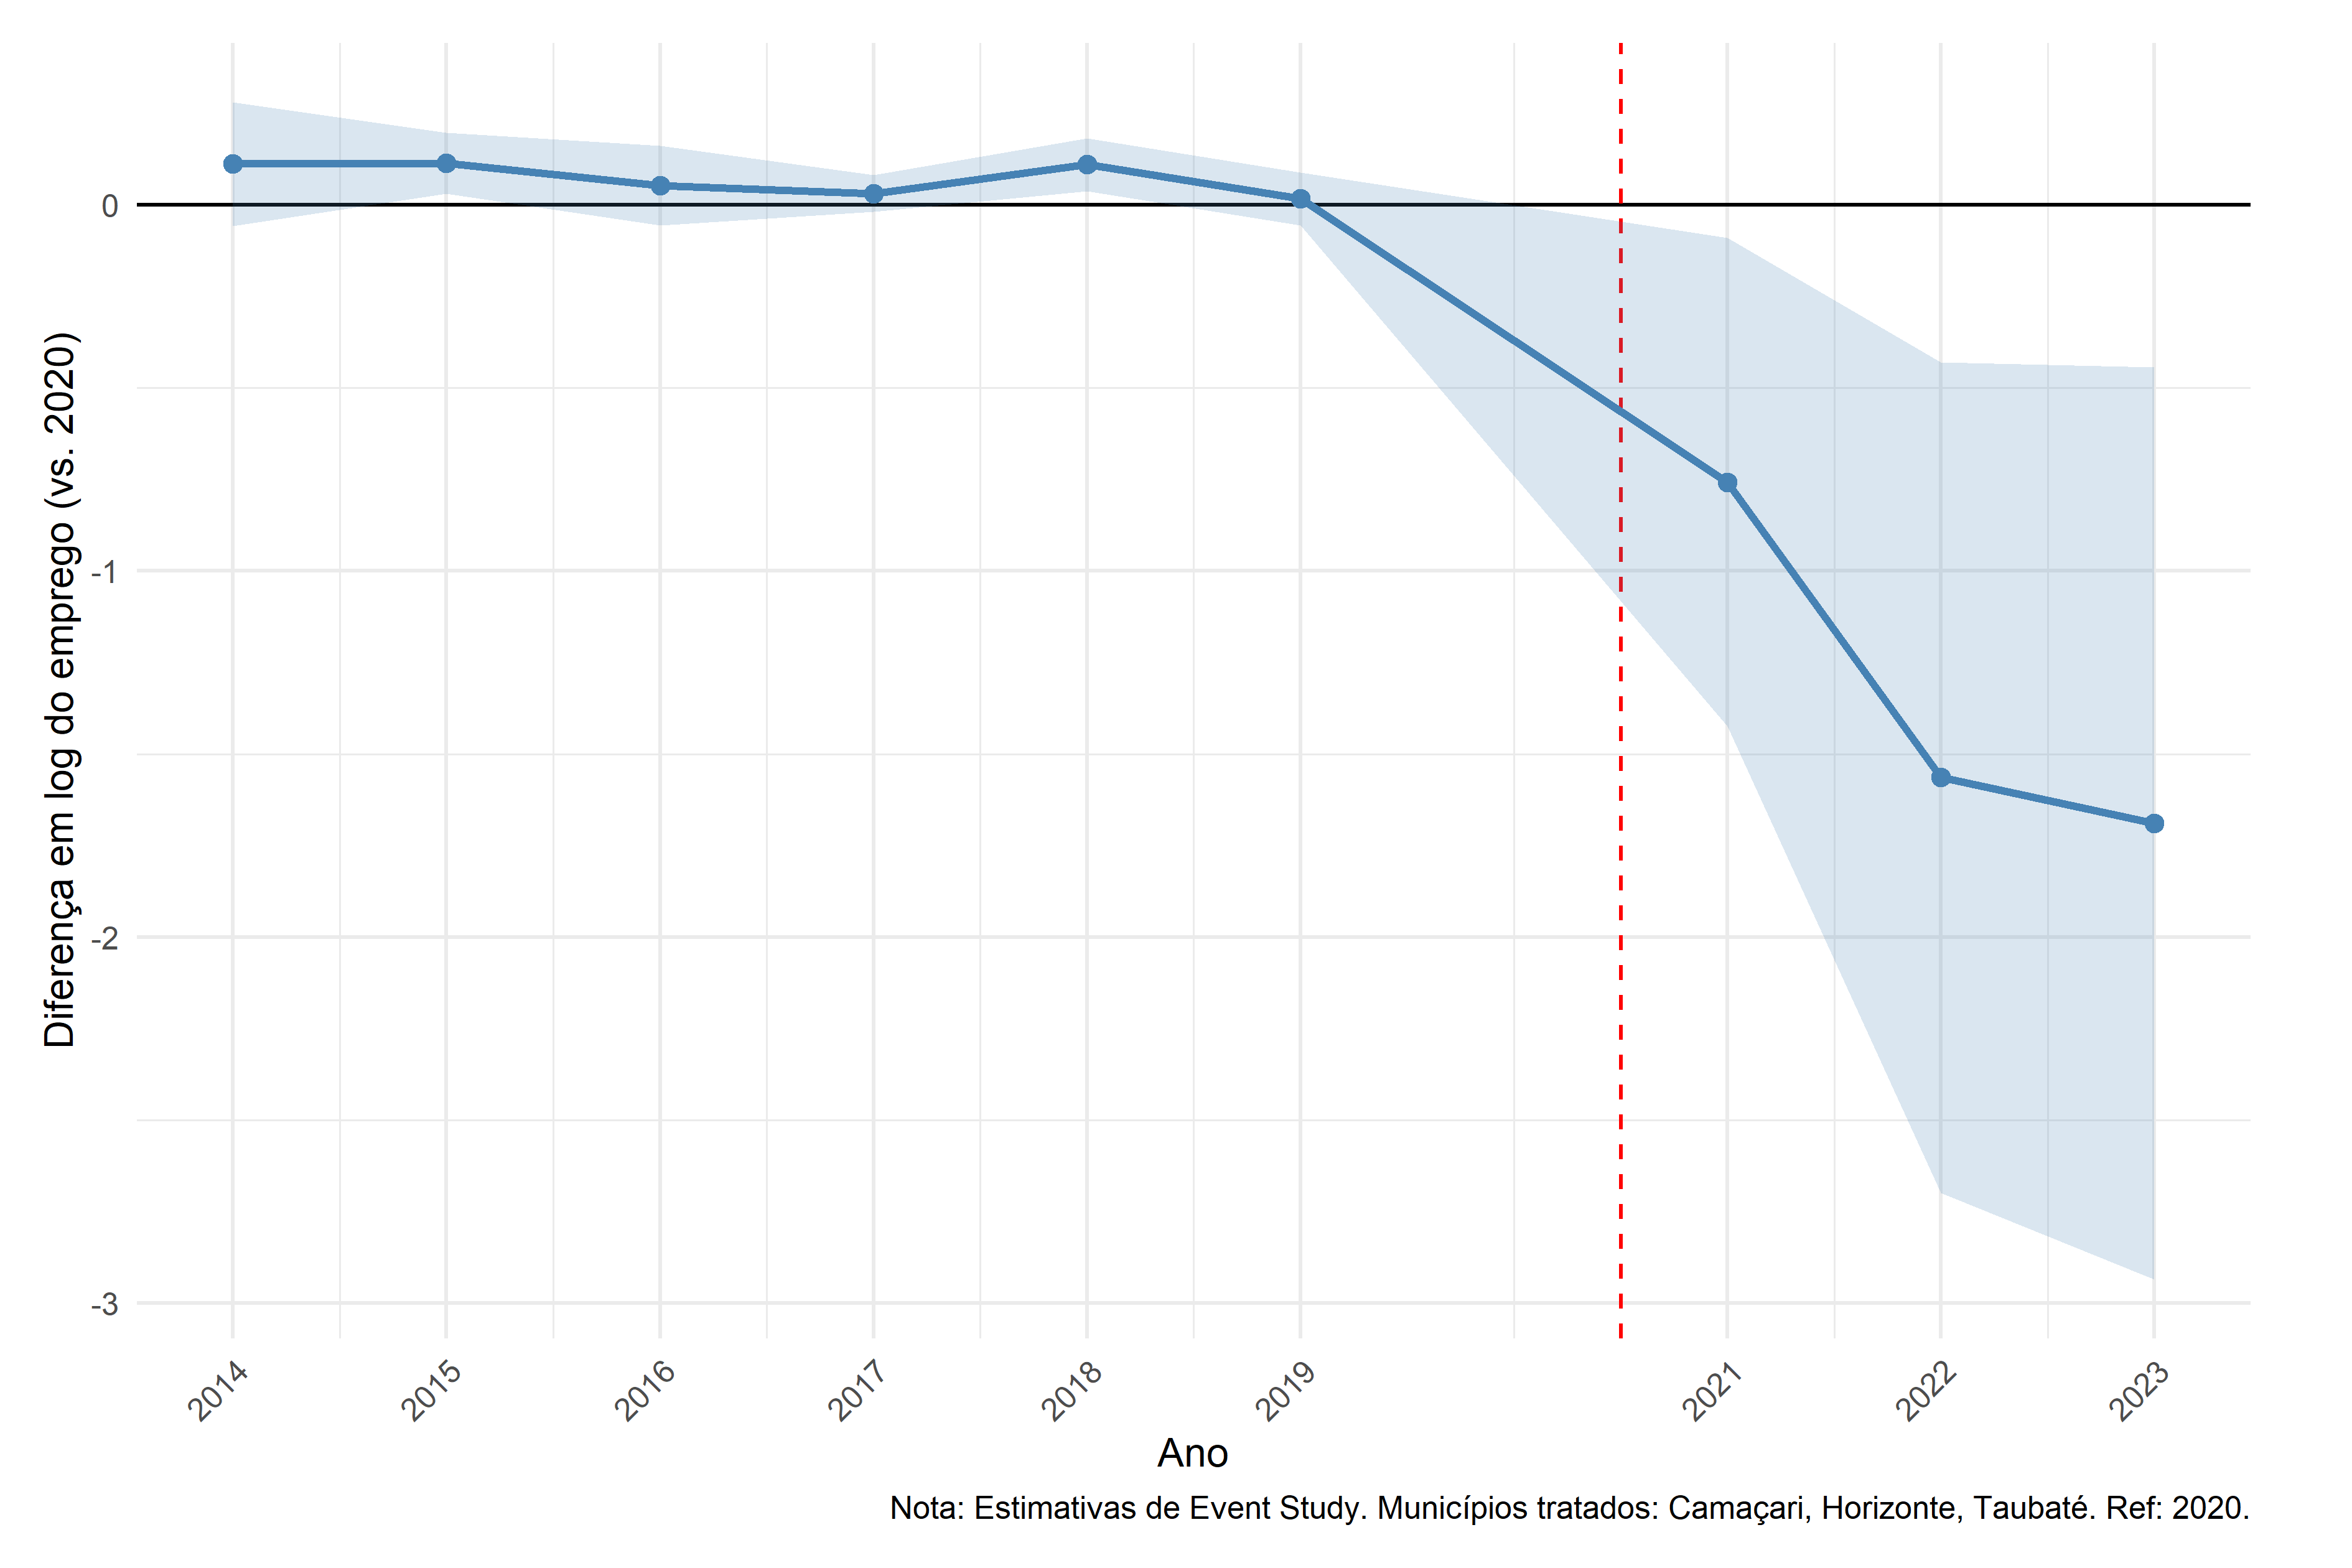
\includegraphics[width=\textwidth]{figuras/EventStudy_420dpi.png}
  \caption{Estudo de evento: efeitos din\^amicos do choque (DDD com efeitos fixos).
    Ano de refer\^encia: 2020. Munic\'ipios tratados: Cama\c{c}ari, Taubat\'e, Horizonte.
    Estimadores \textit{clustered} por munic\'ipio. Banda de 95\% de confian\c{c}a.}
  \label{fig:eventstudy}
\end{figure}

Observa-se que os coeficientes do pr\'e-tratamento permanecem pr\'oximos de zero e sem trajet\'oria sistem\'atica, o que \'e compat\'ivel com a aus\^encia de din\^amica diferencial imediatamente anterior ao choque. A partir de 2021, os coeficientes tornam-se negativos e permanecem nesse patamar nos anos seguintes, sugerindo persist\^encia do efeito no horizonte observado (2021--2023). No presente desenho, a data de choque comum aos tratados reduz preocupa\c{c}\~oes associadas a compara\c{c}\~oes entre coortes \parencite{sun2021}, mas a leitura do estudo de evento permanece como evid\^encia complementar, ancorada na especifica\c{c}\~ao DDD e nos placebos.

\subsection{An\'alise espacial: efeitos diretos e de transbordamento}
\label{sub:espacial}

A especifica\c{c}\~ao SLX-DDD descrita na Se\c{c}\~ao~\ref{sub:slxddd} (Eq.~\ref{eq:slxddd}) \'e estimada para o setor automotivo com o objetivo de verificar se o choque gerado pelo encerramento das opera\c{c}\~oes da Ford se propagou al\'em das fronteiras municipais dos tr\^es munic\'ipios diretamente afetados. A an\'alise \'e motivada pela hip\'otese de que a desorganiza\c{c}\~ao das cadeias de fornecimento pode ter gerado efeitos negativos sobre munic\'ipios vizinhos que mantinham v\'inculos produtivos com as plantas encerradas, especialmente naqueles com presen\c{c}a de fornecedores de autopeças e prestadores de servi\c{c}os industriais. Os resultados s\~ao apresentados na Tabela~\ref{tab:slx_auto}.

\begin{longtable}{p{8.5cm}cccc}
\caption{SLX-DDD: efeitos direto e de transbordamento sobre o complexo automotivo}
\label{tab:slx_auto} \\
\toprule
Coeficiente & Estimativa & EP & $t$ & $p$-valor \\
\midrule
\endfirsthead
\multicolumn{5}{c}{{\tablename\ \thetable{} -- continua\c{c}\~ao}} \\
\toprule
Coeficiente & Estimativa & EP & $t$ & $p$-valor \\
\midrule
\endhead
\midrule
\multicolumn{5}{r}{{\footnotesize Continua na pr\'oxima p\'agina}} \\
\endfoot
\bottomrule
\multicolumn{5}{l}{\footnotesize 261.660 obs. EF: $\alpha_{mt}$, $\gamma_{st}$, $\delta_{ms}$. EP agrupado por munic\'ipio. ** $p<0{,}01$. Elabora\c{c}\~ao pr\'opria.}\\
\endlastfoot
$\hat{\beta}_1$: efeito direto (munic\'ipios tratados) & $-1{,}4021$ & $0{,}477$ & $-2{,}94$ & $0{,}003$** \\
$\hat{\beta}_2$: transbordamento (vizinhos) & $-0{,}2272$ & $0{,}184$ & $-1{,}23$ & $0{,}218$ \\
\end{longtable}

O efeito direto ($\hat{\beta}_1 = -1{,}402$; $p = 0{,}003$) \'e virtualmente id\^entico ao DDD de base, confirmando a robustez do resultado principal \`a inclus\~ao do componente espacial. O efeito de transbordamento automotivo para munic\'ipios vizinhos n\~ao \'e estatisticamente significativo ($\hat{\beta}_2 = -0{,}227$; $p = 0{,}218$), indicando que o choque foi absorvido principalmente pelas localidades diretamente afetadas, sem propaga\c{c}\~ao expressiva no setor automotivo para o entorno imediato.


\subsection{Testes de robustez: placebos temporal e espacial}
\label{sub:robustez_result}

Os testes placebo refor\c{c}am a interpreta\c{c}\~ao causal do resultado principal ao avaliar se efeitos semelhantes emergem: (a) em anos artificiais pr\'e-2021 (placebo temporal) e (b) sob reatribui\c{c}\~ao aleat\'oria do tratamento no espa\c{c}o (placebo espacial por permuta\c{c}\~ao).

No placebo temporal, desloca-se artificialmente o ano do choque para anos estritamente pr\'e-2021 e reestima-se a especifica\c{c}\~ao principal em janelas do pr\'e-tratamento. A Tabela~\ref{tab:placebo_temporal} apresenta os coeficientes placebo v\'alidos, os quais s\~ao pequenos em magnitude e n\~ao estatisticamente significativos, sustentando que a estimativa principal n\~ao est\'a capturando uma din\^amica diferencial preexistente.

\begin{longtable}{@{}lcc@{}}
\caption{Resultados do placebo temporal.}
\label{tab:placebo_temporal} \\
\toprule
Ano placebo & Coeficiente ($\hat{\beta}^{(p)}$) & Significativa? \\
\midrule
\endfirsthead
\multicolumn{3}{c}{{\tablename\ \thetable{} -- continua\c{c}\~ao}} \\
\toprule
Ano placebo & Coeficiente ($\hat{\beta}^{(p)}$) & Significativa? \\
\midrule
\endhead
\midrule
\multicolumn{3}{r}{{\footnotesize Continua na pr\'oxima p\'agina}} \\
\endfoot
\bottomrule
\multicolumn{3}{l}{\footnotesize Fonte: Elabora\c{c}\~ao pr\'opria.}\\
\endlastfoot
2016 & $-0{,}0705$ & N\~ao \\
2017 & $-0{,}0128$ & N\~ao \\
2018 & $+0{,}0207$ & N\~ao \\
2019 & $-0{,}0623$ & N\~ao \\
\end{longtable}

No placebo espacial por permuta\c{c}\~ao de Fisher ($B = 2.000$), reatribui-se repetidas vezes o conjunto de munic\'ipios tratados dentro de um \textit{pool} de munic\'ipios compar\'aveis e obt\'em-se uma distribui\c{c}\~ao emp\'irica do estimador. A Figura~\ref{fig:placebo_espacial} mostra essa distribui\c{c}\~ao e a posi\c{c}\~ao do coeficiente real.

\begin{figure}[!ht]
  \centering
  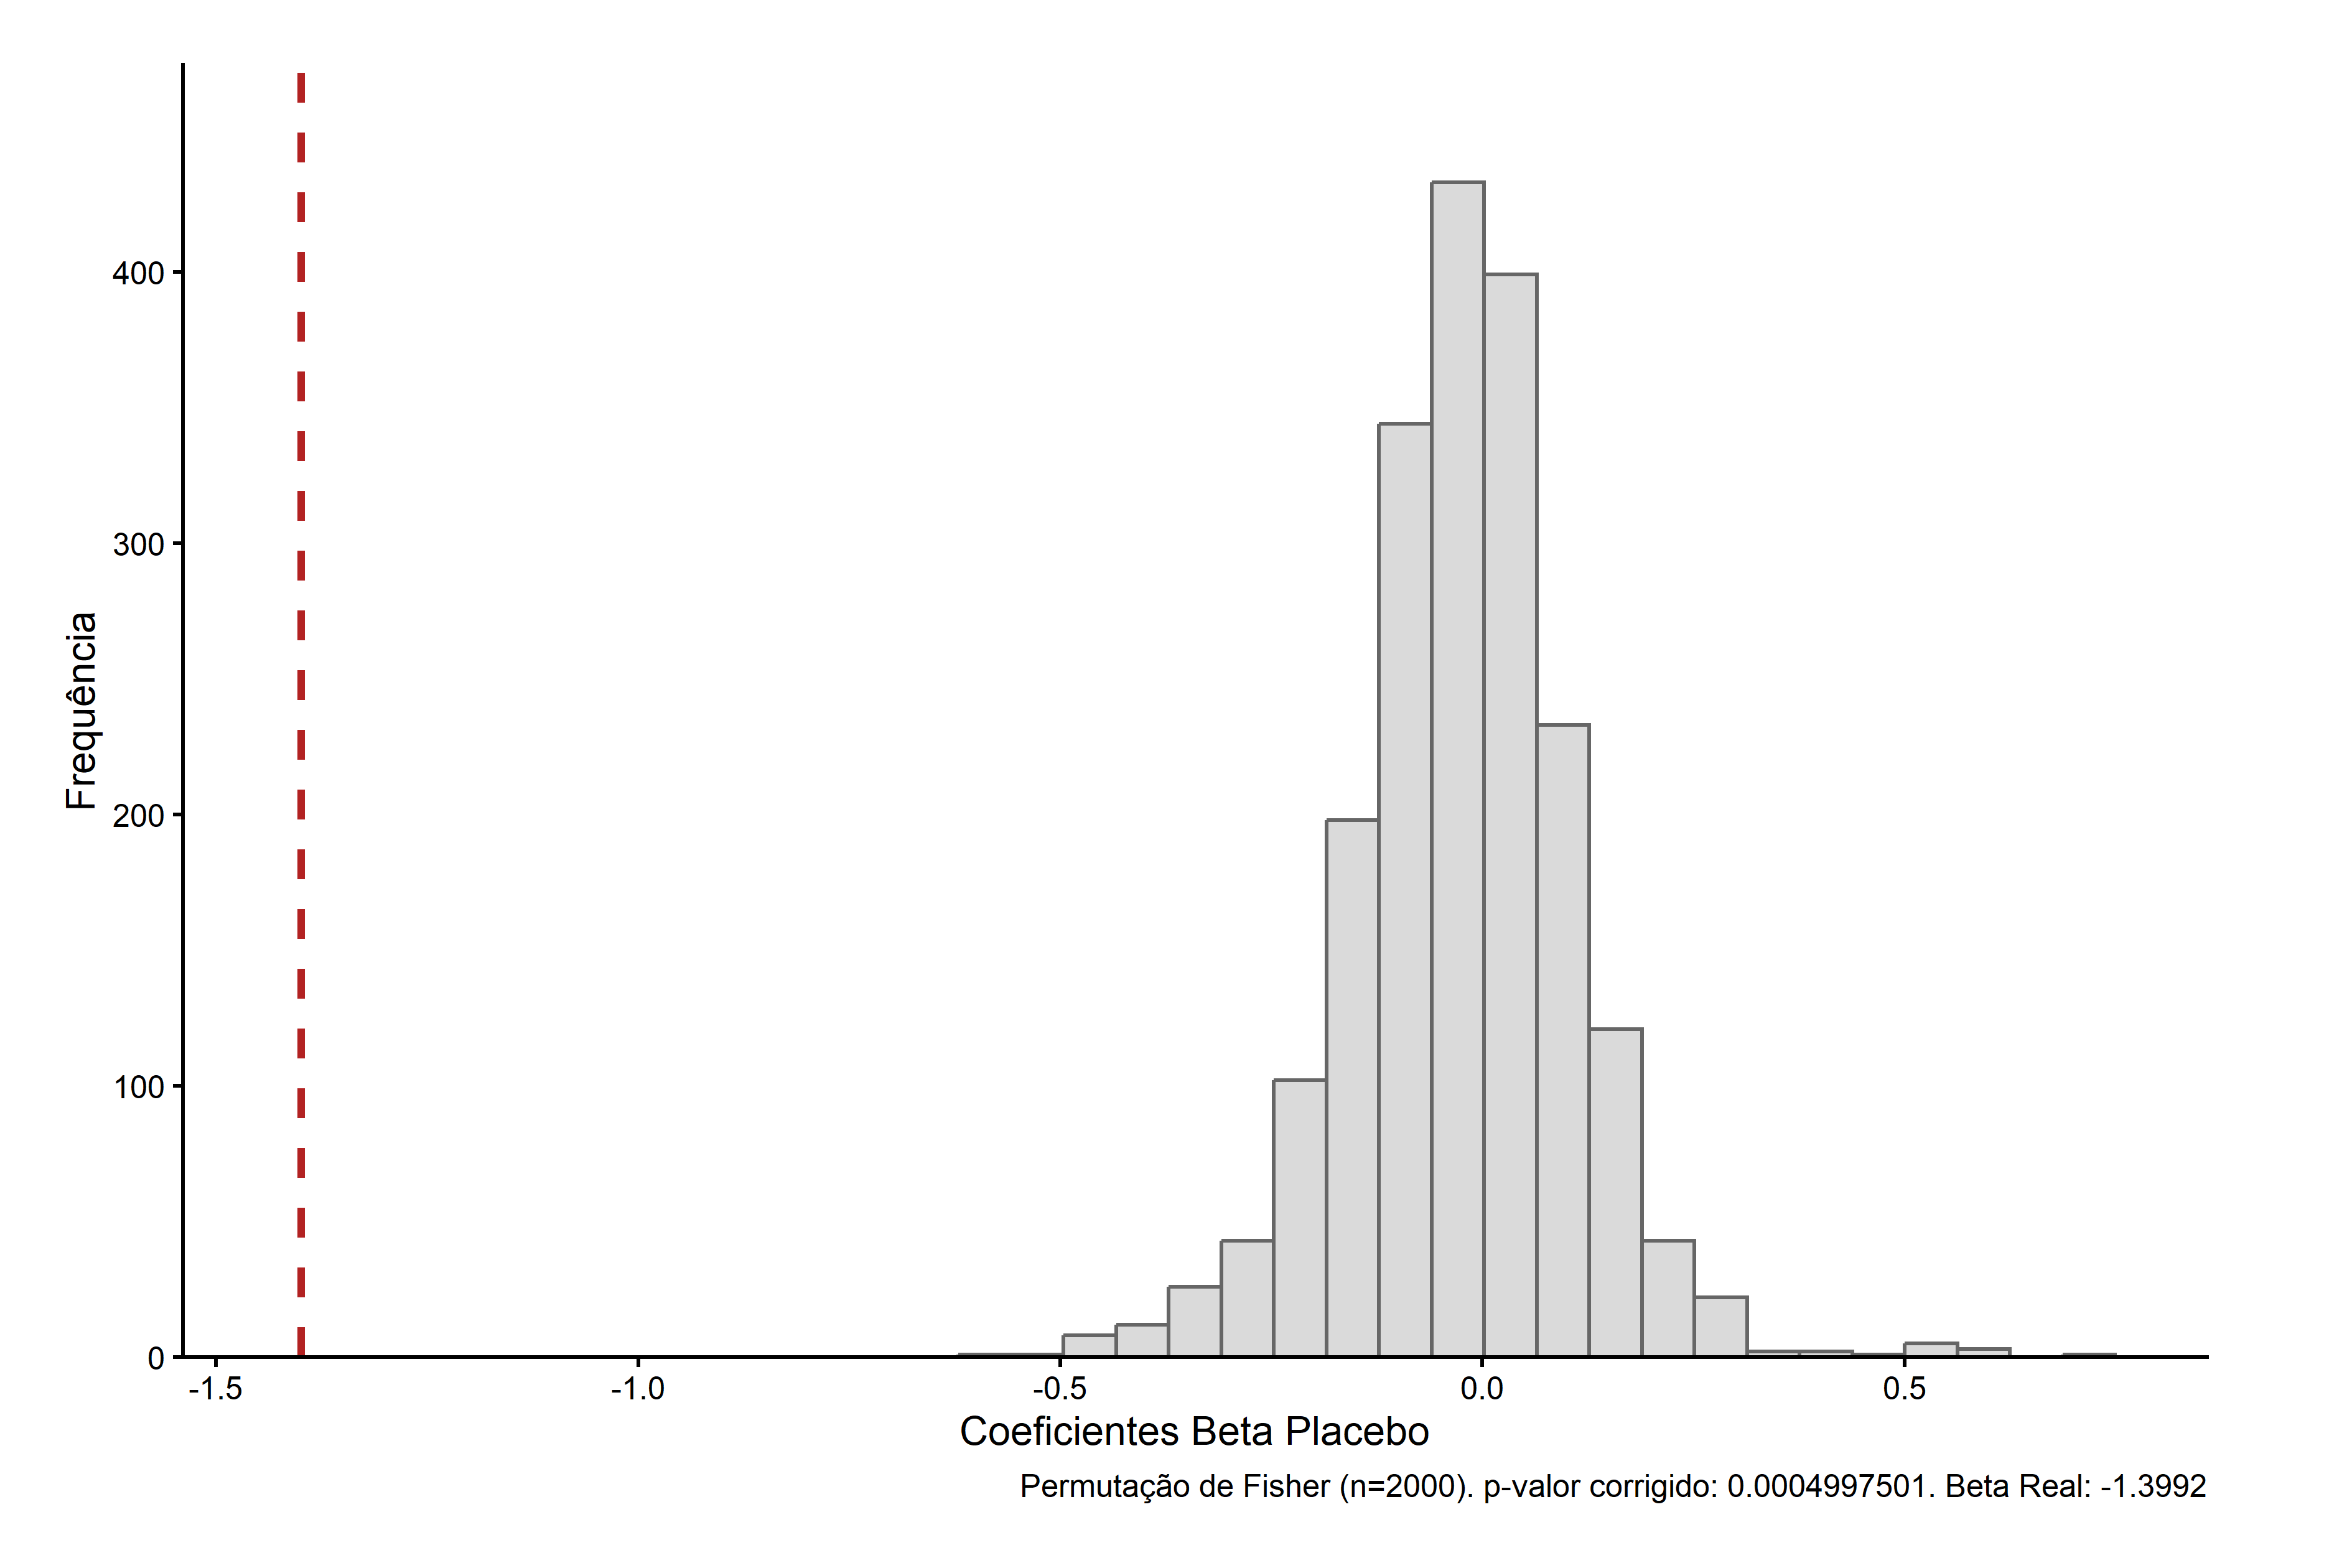
\includegraphics[width=\textwidth]{figuras/PlaceboEspacial_420dpi.png}
  \caption{Placebo espacial: distribui\c{c}\~ao de $\hat{\beta}^{(b)}$ das permuta\c{c}\~oes de
    Fisher ($B = 2.000$). Linha vermelha tracejada: coeficiente real.
    $p$-valor corrigido $\approx 0{,}0005$.}
  \label{fig:placebo_espacial}
\end{figure}

O $p$-valor emp\'irico aproximado de 0,0005 indica que um efeito t\~ao negativo quanto o estimado \'e extremamente improv\'avel sob reatribui\c{c}\~oes aleat\'orias do tratamento no espa\c{c}o, refor\c{c}ando que o resultado n\~ao parece ser uma realiza\c{c}\~ao at\'ipica de varia\c{c}\~ao esp\'uria do painel. Em termos pr\'aticos, apenas 1 permuta\c{c}\~ao em cada 2.000 produziu um coeficiente t\~ao negativo quanto o observado para os munic\'ipios realmente afetados pela sa\'ida da Ford, o que fornece evid\^encia n\~ao param\'etrica forte de que a localiza\c{c}\~ao espec\'ifica do tratamento \'e determinante para a magnitude do impacto estimado. Esse resultado \'e consistente com a hip\'otese de que a vulnerabilidade dos munic\'ipios tratados n\~ao \'e apenas fruto de caracter\'isticas geogr\'aficas gen\'ericas, mas da depend\^encia estrutural de sua base produtiva em rela\c{c}\~ao ao complexo automotivo.

Em s\'intese, a combina\c{c}\~ao da estimativa DDD com efeitos fixos de alta dimens\~ao, da an\'alise din\^amica por estudo de evento e dos testes de placebo temporal e espacial converge de forma coerente para a conclus\~ao de que o encerramento das opera\c{c}\~oes da Ford constituiu um choque econ\^omico local de grande magnitude, com impacto negativo substancial e persistente sobre o emprego formal no setor automobilist\'ico dos munic\'ipios diretamente expostos. A consist\^encia dos resultados atrav\'es de m\'ultiplos estimadores e m\'ultiplos testes de validade refor\c{c}a a robustez da infer\^encia causal apresentada.

% ============================================================
\subsection{Robustez: Estimadores Alternativos e Justificativa do Modelo Principal}
\label{sec:robustez_modelos}

O DDD com efeitos fixos de alta dimens\~ao \'e o estimador principal por combinar tr\^es vantagens: a tripla diferen\c{c}a remove confundidores temporais, espaciais e setoriais que o DD convencional n\~ao elimina \parencite{olden2022,berck2016}; os tr\^es conjuntos de efeitos fixos absorvem toda heterogeneidade observ\'avel e n\~ao observ\'avel ao n\'ivel munic\'ipio-ano, setor-ano e munic\'ipio-setor \parencite{wooldridge2010}; e a coorte \'unica de tratamento ($T_0 = 2021$) afasta preocupa\c{c}\~oes com contamina\c{c}\~ao entre coortes \parencite{sun2021,callaway2021}. Os demais estimadores s\~ao empregados como testes de robustez: o DDD Espacial incorpora transbordamento espacial; o DD Simples avalia a magnitude sem controle intersetorial; Sun e Abraham \parencite{sun2021} e Callaway e Sant'Anna \parencite{callaway2021} utilizam pond\'era\c{c}\~ao por coorte e estimador duplamente robusto; e o SDID \parencite{arkhangelsky2021} valida o resultado via correspond\^encia sint\'etica pr\'e-tratamento. A Tabela~\ref{tab:robustez} reporta os coeficientes, erros-padr\~ao e efeito percentual $\%\Delta\text{Emp} = 100\cdot(e^{\hat{\tau}}-1)$ para cada especifica\c{c}\~ao.

\begin{longtable}{lcccc}
\caption{Robustez: compara\c{c}\~ao de estimadores do efeito da sa\'ida da Ford sobre o emprego automotivo formal}
\label{tab:robustez} \\
\toprule
\textbf{Modelo} & $\hat{\tau}$ & EP & $p$-valor & $\%\Delta\text{Emp}$ \\
\midrule
\endfirsthead
\multicolumn{5}{c}{{\tablename\ \thetable{} -- continua\c{c}\~ao}} \\
\toprule
\textbf{Modelo} & $\hat{\tau}$ & EP & $p$-valor & $\%\Delta\text{Emp}$ \\
\midrule
\endhead
\midrule
\multicolumn{5}{r}{{\footnotesize Continua na pr\'oxima p\'agina}} \\
\endfoot
\bottomrule
\endlastfoot
\textit{Modelo principal} & & & & \\
\quad DDD + EF              & $-1{,}3992$ & $0{,}477$ & $0{,}003$** & $-75{,}3\%$ \\
\midrule
\textit{Testes de robustez} & & & & \\
\quad DDD Espacial (direto) & $-1{,}4021$ & $0{,}477$ & $0{,}003$** & $-75{,}4\%$ \\
\quad DD Simples            & $-1{,}3689$ & $0{,}472$ & $0{,}004$** & $-74{,}6\%$ \\
\quad Sun \& Abraham        & $-1{,}3286$ & $0{,}476$ & $0{,}005$** & $-73{,}6\%$ \\
\quad Callaway \& Sant'Anna & $-1{,}3286$ & $0{,}567$ & $0{,}020$*  & $-73{,}6\%$ \\
\quad SDID                  & $-1{,}3476$ & $0{,}706$ & $\dagger$   & $-74{,}0\%$ \\
\end{longtable}
\noindent\begin{minipage}{0.96\textwidth}
\footnotesize
\textit{Notas:} EP = erro-padr\~ao. DDD+EF, DDD Espacial, DD Simples e Sun \& Abraham: EP agrupado por munic\'ipio. Callaway \& Sant'Anna: EP \textit{bootstrap} (999 itera\c{c}\~oes). SDID: EP \textit{jackknife}. $\dagger$ $t = -1{,}91$; o EP \textit{jackknife} \'e conservador com $N_{\text{tratados}} = 3$ unidades; a signific\^ancia n\~ao param\'etrica \'e confirmada pelo placebo de Fisher ($p \approx 0{,}0005$). $*p < 0{,}05$; $**p < 0{,}01$. Todos os modelos: $T_0 = 2021$, ano de refer\^encia 2020, setor automotivo (CNAE C.A.\ e G.A.). Elabora\c{c}\~ao pr\'opria.
\end{minipage}
\vspace{0.5\baselineskip}

Os seis estimadores convergem em uma faixa de apenas 1{,}8 pontos percentuais ($-73{,}6\%$ a $-75{,}4\%$), abarcando m\'etodos com premissas de identifica\c{c}\~ao fundamentalmente distintas. Essa consist\^encia transversal indica que o resultado n\~ao \'e artefato de uma \'unica escolha de especifica\c{c}\~ao. O DDD Espacial ($\hat{\tau} = -1{,}402$) replica virtualmente o DDD de base, confirmando que o transbordamento automotivo n\~ao contamina a estimativa. O DD Simples ($\hat{\tau} = -1{,}369$) sugere que a ``terceira diferen\c{c}a'' intersetorial acrescenta rigor metodol\'ogico sem alterar substancialmente a magnitude. A leve redu\c{c}\~ao de Sun e Abraham e Callaway e Sant'Anna ($\hat{\tau} = -1{,}329$) reflete a aus\^encia de heterogeneidade entre coortes relevante neste painel de coorte \'unica. O SDID ($\hat{\tau} = -1{,}348$), que n\~ao imp\~oe estrutura param\'etrica de efeitos fixos, constitui a prova de robustez mais independente de premissas param\'etricas.

% ============================================================
\section{Considera\c{c}\~oes Finais}
\label{sec:conclusao}

Este artigo estimou o efeito do encerramento das opera\c{c}\~oes industriais da Ford no Brasil em 2021 sobre o emprego formal do complexo automotivo em tr\^es munic\'ipios diretamente expostos (Cama\c{c}ari, Taubat\'e e Horizonte), utilizando microdados da RAIS no per\'iodo de 2014 a 2023 e um desenho de Diferen\c{c}as em Diferen\c{c}as Tripla (DDD) com efeitos fixos de alta dimens\~ao. A evid\^encia emp\'irica aponta para um impacto negativo, estatisticamente significativo e de grande magnitude: $\hat{\beta} = -1{,}3992$ ($p < 0{,}01$), equivalente a uma redu\c{c}\~ao de aproximadamente $75\%$ no emprego setorial formal, estimado em rela\c{c}\~ao a um contrafactual disciplinado simultaneamente por varia\c{c}\~ao temporal, espacial e setorial.

A leitura do resultado principal deve enfatizar seu car\'ater l\'iquido e relativo: o estimador DDD desconta choques comuns no tempo, choques setoriais agregados e condi\c{c}\~oes locais que afetam m\'ultiplos setores. Embora a evid\^encia descritiva do grupo tratado confirme queda acentuada dos v\'inculos setoriais a partir de 2021 (de 16.528 em 2020 para 10.392 em 2021, mantendo-se abaixo de 10.100 at\'e 2023), o coeficiente DDD quantifica a parte do ajuste que permanece ap\'os controlar por essas fontes de heterogeneidade. A an\'alise din\^amica via estudo de evento \'e compat\'ivel com essa interpreta\c{c}\~ao: os coeficientes pr\'e-tratamento s\~ao pr\'oximos de zero sem tend\^encia sistem\'atica, e a persist\^encia p\'os-choque fica evidente pela amplia\c{c}\~ao do efeito entre 2021 ($\hat{\mu} \approx -0{,}75$) e 2022--2023 ($\hat{\mu} \approx -1{,}57$ a $-1{,}66$), consistente com a propaga\c{c}\~ao de efeitos multiplicadores ao longo da cadeia produtiva.

A an\'alise espacial via modelo SLX-DDD confirmou que o efeito direto sobre os munic\'ipios tratados \'e praticamente id\^entico ao DDD de base ($\hat{\beta}_1 = -1{,}402$; $p < 0{,}01$), sem transbordamento estatisticamente significativo do setor automotivo para munic\'ipios vizinhos. Esse resultado indica que o choque foi absorvido principalmente pelas localidades diretamente afetadas, sem propaga\c{c}\~ao expressiva para o entorno imediato no complexo automotivo.

Os exerc\'icios de robustez contribuem para qualificar a solidez dos achados em dois n\'iveis. Os placebos temporais no per\'iodo pr\'e-2021 n\~ao produzem estimativas estatisticamente relevantes, e o placebo espacial por permuta\c{c}\~ao de Fisher posiciona o coeficiente real na regi\~ao extrema da distribui\c{c}\~ao emp\'irica ($p \approx 0{,}0005$). Al\'em disso, seis estimadores com premissas de identifica\c{c}\~ao distintas (DDD+EF, DDD Espacial, DD Simples, Sun \& Abraham, Callaway \& Sant'Anna e SDID) convergem para uma faixa estreita de $-73{,}6\%$ a $-75{,}4\%$. Essa consist\^encia transversal, especialmente o alinhamento do SDID (que n\~ao imp\~oe estrutura param\'etrica de efeitos fixos) com o DDD de base, constitui evid\^encia forte de que o resultado n\~ao \'e artefato de uma \'unica escolha de especifica\c{c}\~ao.

As conclus\~oes devem ser interpretadas no escopo do que os dados e o desenho identificam: trata-se de um efeito sobre o emprego formal setorial no n\'ivel municipal, sem pretens\~ao de medir diretamente renda, bem-estar, informalidade ou outros desfechos n\~ao observados na RAIS. A aus\^encia de informa\c{c}\~ao sobre ocupa\c{c}\~ao, sal\'ario e condi\c{c}\~ao de atividade nos microdados da RAIS restringe a infer\^encia ao estoque de v\'inculos formais, n\~ao capturando poss\'iveis realoca\c{c}\~oes para o setor informal ou para outros munic\'ipios.

Como agenda de pesquisa, os resultados sugerem tr\^es extens\~oes principais. Primeiro, aprofundar o mapeamento do ajuste p\'os-choque distinguindo mudan\c{c}as de composi\c{c}\~ao setorial e ocupacional, de modo a identificar quais categorias de trabalhadores absorveram desproporcionalmente o ajuste. Segundo, avaliar os efeitos sobre informalidade e renda utilizando fontes complementares, como a PNAD Cont\'inua e registros administrativos fiscais, para capturar transbordamentos ao mercado informal. Terceiro, explorar a heterogeneidade entre os tr\^es munic\'ipios tratados, dado que Cama\c{c}ari, Taubat\'e e Horizonte diferem em porte, diversifica\c{c}\~ao setorial e grau de depend\^encia da cadeia automotiva. A baixa cardinalidade do grupo tratado imp\~oe cautela na extrapola\c{c}\~ao para outros epis\'odios, mas a coer\^encia dos resultados com a literatura internacional sobre fechamentos de plantas industriais \parencite{jofremonseny2018,beer2019,chapain2008} reforca a plausibilidade dos achados e reafirma a relev\^ancia do instrumento anal\'itico adotado para a avalia\c{c}\~ao de choques econ\^omicos locais.

% ============================================================
\printbibliography

\end{document}
